%\addtorecentlist{secnumdepth}

\begin{saveblock}{standalone}
    \begin{highlightblock}[linewidth=\textwidth,gobble=8]
        % Bestand: prachtigeformule.tex
        \documentclass{standalone}
        \usepackage{amsmath,amssymb}

        \begin{document}
            $\displaystyle\sum_{k=0}^{\infty}
            \frac{x^k}{k!}=e^{x}$
        \end{document}
    \end{highlightblock}
\end{saveblock}

\begin{frame}
    \frametitle{Standalone}

    \centering

    \useblock{standalone}

    \hll|\\includegraphics[...]\{prachtigeformule.pdf\}|

    \medskip
    \adjustbox{cfbox=black 1pt 0pt}{%
    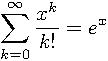
\includegraphics[width=\linewidth,height=40pt,keepaspectratio]{assets/document-standalone.pdf}%
    }
    
    % \begin{columns}
    %     \begin{column}{0.5\textwidth}
    %         \useblock{standalone}
    %     \end{column}
    %     \begin{column}{0.5\textwidth}
    %         \hll|\\includegraphics[...]\{standalone.pdf\}|

    %         \medskip
    %         \adjustbox{cfbox=black 1pt 0pt}{%
    %         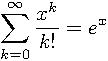
\includegraphics[width=\linewidth,height=0.8\textheight,keepaspectratio]{assets/document-standalone.pdf}%
    %         }
    %     \end{column}
    % \end{columns}
\end{frame}

\begin{frame}
    \includegraphics[width=\textwidth,height=0.8\textheight,keepaspectratio]{assets/.jpg}
\end{frame}

\begin{frame}
    formulaArt.pdf
\end{frame}

\begin{frame}
    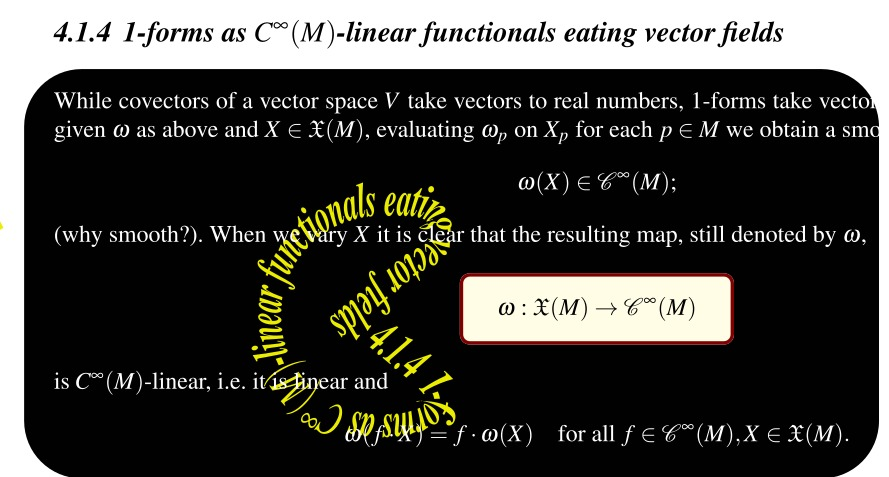
\includegraphics[width=\textwidth,height=0.8\textheight,keepaspectratio]{assets/pacman.jpg}
\end{frame}
